% Please use the skeleton file you have received in the 
% invitation-to-submit email, where your data are already
% filled in. Otherwise please make sure you insert your 
% data according to the instructions in PoSauthmanual.pdf
\documentclass{PoS}

\usepackage{subfigure}
% \usepackage{cite} --> non fa vedere i link
% \usepackage{hyperref} --> non funziona

\newcommand{\ptjet}{\ensuremath{{p}_{T}^{\mathrm jet}}}
\newcommand{\antikt}{anti-$k_t$}

\title{Searches for Heavy Hadronic Resonances with the ATLAS and CMS detectors at the LHC}

\ShortTitle{Hadronic resonances at the LHC}

\author{\speaker{Caterina Doglioni}\\%\thanks{A footnote may follow.}\\
        University of Geneva\\
        E-mail: \email{caterina.doglioni@cern.ch}}

\author{\speaker{Francesco Santanastasio}\\
       CERN\\
       E-mail: \email{francesco.santanastasio@cern.ch}}

\abstract{..........................\
          ...........................}

\FullConference{VI Italian workshop on p-p physics at the LHC,\\
		8-10 May 2013\\
		Acquario di Genova, Ponte Spinola, Area Porto Antico, Genova, Italy}


\begin{document}

\section{Introduction}
New resonances, that couples to quarks and gluons and decay to final states with hadronic jets, 
can be produced copiously at the Large Hadron Collider (CERN). 
%The large cross section of processes decaying in quarks and gluons 
%at the Large Hadron Collider makes searches for new, heavy resonances decaying 
%into hadronic jets an attractive ground to test the validity of the Standard Model 
%to the highest energy scales. 
This review outlines a selection of searches for heavy resonances in hadronic final states 
performed at the ATLAS and CMS experiments using the proton-proton collision data collected 
at a center-of-mass energy of 7 TeV (2011) and 8 TeV (2012). A series of points that 
are deemed important for current and future searches are also discussed.

%\section{Jet reconstruction and calibration: da tagliare?}

%Both ATLAS and CMS employ similar algorithms and techniques for jet reconstruction, 
%as most searches employ the \antikt{} jet finding algorithm~\cite{Cacciari:2008gp},
%although the inputs for jet finding are different. ATLAS uses energy deposits from the calorimeters,
%while CMS complements the calorimeter information with measurements of particle momenta
%from the inner detector. The hadronic energy scale is calibrated using a series of corrections 
%derived both from Monte-Carlo simulation and from 
%data~\cite{ATLAS-CONF-2013-004, 1748-0221-6-11-P11002, Aad:2011he}. 
%The jet energy scale uncertainty, which dominates among the sources of systematic 
%uncertainty for most of the searches described in this review, is derived using data-driven 
%techniques and has a similar magnitude across
%jet transverse momenta $p_\mathrm{T}$ and pseudorapidities $\eta$ for the two experiments. 
%However, as it can be noted in Figure~\ref{Fig:JESUnc}, 
%the estimate of the uncertainty for jets above 2~TeV differs between ATLAS and CMS.  

%\begin{figure}[b]
%\subfigure[ATLAS jet energy scale uncertainty]
%{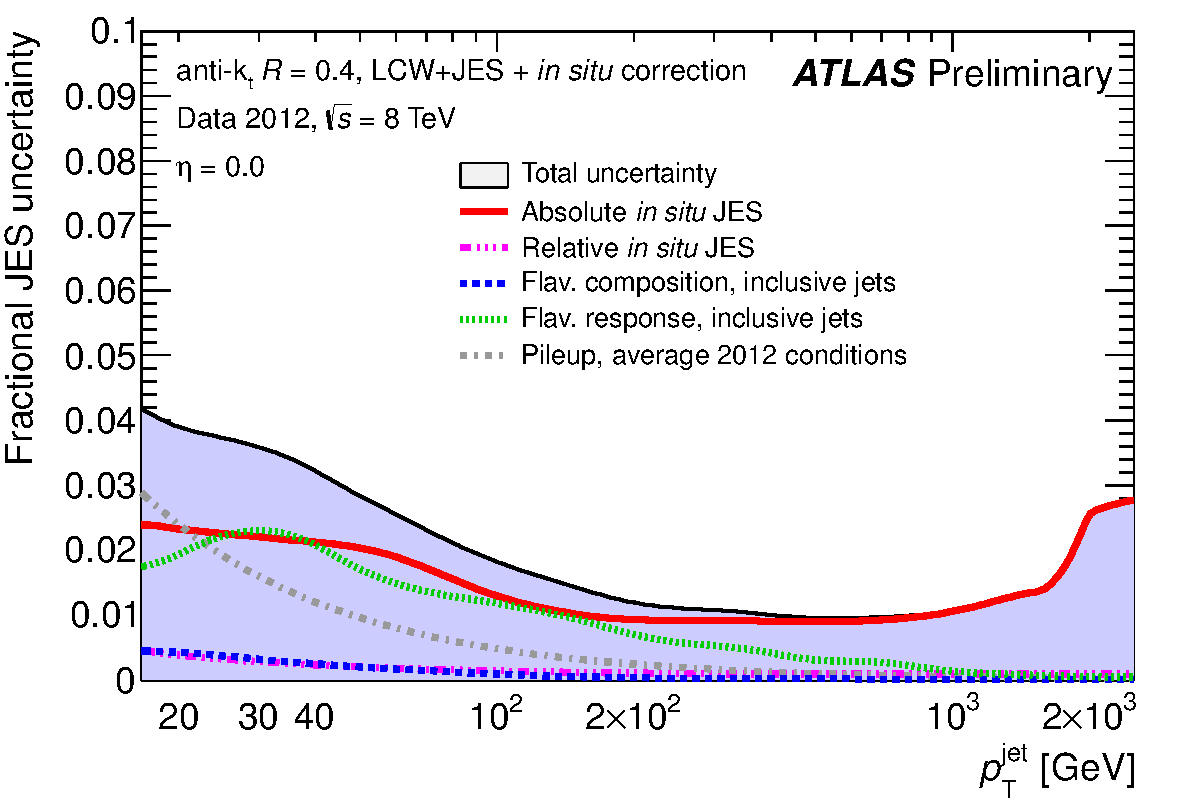
\includegraphics[width=0.58\textwidth]{Figure/ATLASJES.pdf}}
%\subfigure[CMS jet energy scale uncertainty]
%{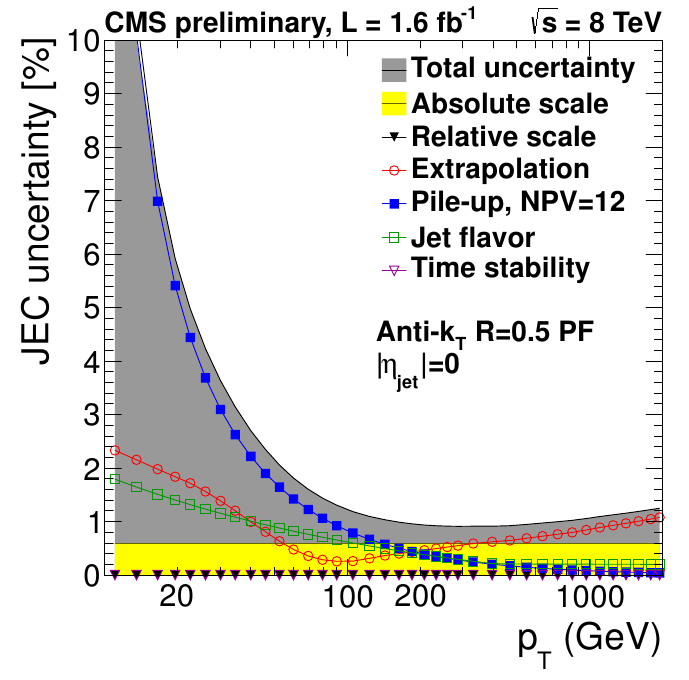
\includegraphics[width=0.4\textwidth]{Figure/CMSJES.png}}
%\caption{Typical jet energy uncertainties for central jets in ATLAS and CMS.}
%\label{Fig:JESUnc}
%\end{figure}

\section{Overview of selected searches in the ATLAS and CMS experiments}

The searches for hadronic resonances can be divided into two main categories:
\begin{itemize}
 \item {\bf Resolved topology} - Searches where the quarks and gluons produced in the final state are each reconstructed at detector level into single,  \textit{resolved} hadronic jets. Examples are the single production of a resonance X decaying to a pair of gluons, or the pair production of two resonances X at rest each decaying to a quark-antiquark pair;
 \item {\bf Boosted topology} - Searches where the quarks and gluons produced in the final state are merged into a single reconstructed jet.  A typical example is the decay of a resonance X into a pair of massive particles Y, with $\mbox{M}_{X} >>\mbox{M}_{Y} $, and Y decays to a pair of light quarks. In this case the resonance Y will be \textit{boosted} 
(the resonance has a large momentum compared to its mass) so that a single hadronic jet with a large distance 
parameter (\textit{wide jet}) encompasses all its decay products. Techniques that exploit the presence of substructure within the \textit{wide jet} are employed to reject background from standard QCD jets and multiple interactions within the same bunch crossing (pile-up). 
\end{itemize}

The quintessential example of hadronic search with resolved jets is the 
search for heavy resonances in the dijet mass distribution. New particles, 
or excitations of quarks indicating 
compositeness,
%further substructure
could manifest 
themselves as narrow 'bumps' in the dijet mass distribution of central leading
and subleading jets above the continuum QCD background~\cite{CMS-PAS-EXO-12-059, ATLAS-CONF-2012-148}. 
The search can be tailored to specific resonances
decaying to heavy quark flavors using $b-$tagging for one or both jets~\cite{CMS-PAS-EXO-12-023}. 
No significant excess over the background has been found for the current ATLAS and CMS analyses,
and lower limits are set on the masses of new particles 
%(Fig.~\ref{Fig:DijetRes}~(a)), 
including model-independent Gaussian resonances of varying width.
%(Fig.~\ref{Fig:DijetRes}~(b)). 
Upper limits on cross section times branching fraction to jets times acceptance of the order of $100$, $10$, and 
$1$~fb at resonance masses of 1.5, 3, and 4.5 TeV, respectively, are set by both experiments.

%\begin{figure}[t]
%\subfigure[CMS limits for various resonances]
%{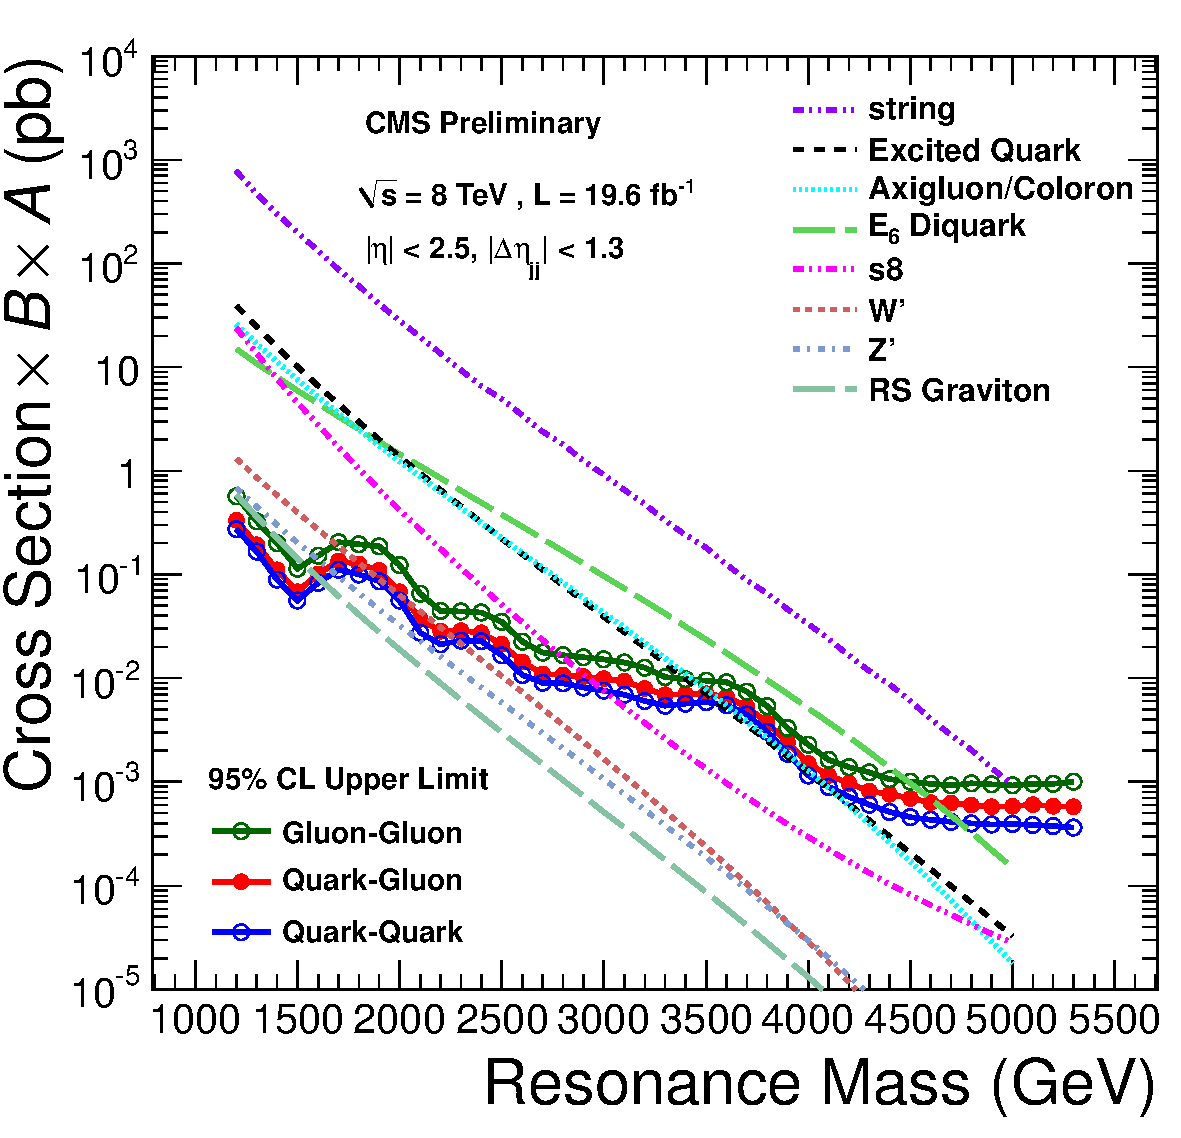
\includegraphics[width=0.48\textwidth]{Figure/DijetCMS.pdf}}
%\subfigure[ATLAS limits on Gaussian resonances]
%{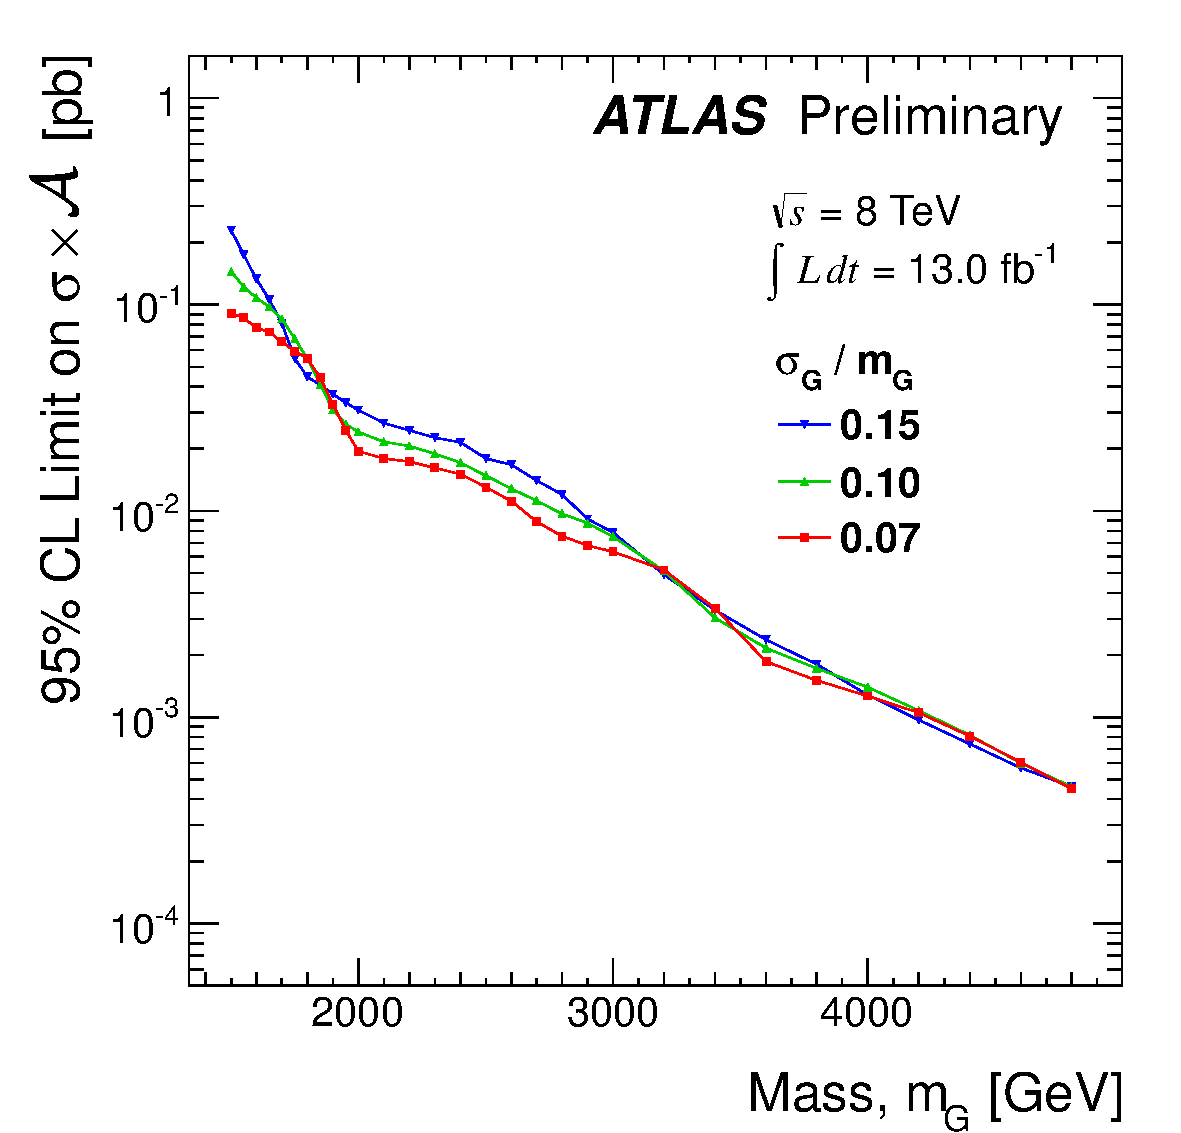
\includegraphics[width=0.48\textwidth]{Figure/DijetGaussATLAS.pdf}}
%\caption{95\% CL limits from dijet mass resonance searches.}
%\label{Fig:DijetRes}
%\end{figure}

Searches for resonances in final states with high jet multiplicity, tailored towards R-Parity Violating supersymmetric 
signatures (such as 3-body decays into quarks of pair produced gluinos, giving a six jet final state), can be performed in both resolved and boosted regimes~\cite{Chatrchyan2012329,SUSYRPVATLAS}.
Both experiments select events with six or more jets, but the background estimation techniques 
for ATLAS and CMS differ. In the resolved channel, ATLAS employs the $p_\mathrm{T}$
of the sixth jet as a discriminant variable, while CMS performs a 'bump-search' in the 
three-jet invariant mass. The combinatorial background (from both the QCD background and the signal)
penalizes the CMS search and allows the ATLAS search to set more stringent limits. A proof-of-principle
boosted jet analysis, although not as sensitive as the resolved one, is also carried on by the ATLAS experiment. 
 
In the case of resonances decaying into pairs of top quarks ($\mbox{t}\bar{\mbox{t}}$) or heavy bosons (WW, ZZ, HH, HZ, ..), 
the use of jet substructure techniques is crucial to achieve a good background rejection. 
In these cases, the tops or heavy bosons coming from a TeV-scale resonance 
are boosted, and therefore their decay products are spatially collimated when reconstructed in the detector.  

Specific techniques for top-tagging, based on the presence of three hard energy deposit corresponding
to the top decay products, have been employed to distinguish top-jets from jets originated from quarks and gluons
that constitute the majority of the QCD background~\cite{Kaplan:2008ie, Plehn:2010st, ATLAS-CONF-2012-065, Almeida:2010pa}. 
Both ATLAS and CMS look for heavy resonances decaying in $t\bar{t}$ at 7 and 8 TeV, in semileptonic and all-hadronic top decays~\cite{TtbarResCMS, TtbarResATLAS, CMS-PAS-B2G-12-005, ATLAS-CONF-2013-052, CMS-PAS-B2G-12-006}.
The ATLAS analysis employes b-tagging to further suppress the QCD background and it sets limits starting from a resonance mass of 500 GeV. The CMS analysis, instead, does not use b-tagging and limits are set starting at a resonance mass of 1 TeV. 
The CMS expected upper limits on the resonance cross section are about a factor 3-4 lower than the ATLAS ones for resonance masses around 2 TeV.  A possible reason might be due to the use of b-tagging: on one side, the b-tag requirement allows the ATLAS analysis to start the search at lower resonance masses compared to CMS, by reducing significantly the QCD background; 
on the other hand, the low b-tag efficiency at high jet pT might penalize the ATLAS search at high resonance masses.

The CMS experiment has also performed a search for RS gravitons decaying to 
WW/ZZ and W'/Z' decaying to Wq/Zq~\cite{Chatrchyan:2012ypy}. This analysis employs 
W/Z-tagging techniques based on the jet mass and the presence
of hard sub-jets to significantly reduce the background and keep a relatively high signal efficiency. 
Given no excesses above background, limits are set on a number benchmark models. 

\section{Discussion points}

\subsection{Jet energy scale in ATLAS and CMS}

Resolved searches in ATLAS and CMS employ the \antikt{} jet finding algorithm~\cite{Cacciari:2008gp}.
% The inputs for jet finding are different: ATLAS uses energy deposits from the calorimeters,
% while CMS complements the calorimeter information with measurements of particle momenta
% from the inner detector. 
The hadronic energy scale is calibrated using a series of corrections 
derived both from Monte-Carlo simulation and from 
data~\cite{ATLAS-CONF-2013-004, 1748-0221-6-11-P11002, Aad:2011he}. 
The jet energy scale uncertainty, which dominates among the sources of systematic 
uncertainty for most of the searches described in this review, is derived using data-driven 
techniques and has a similar magnitude across
jet transverse momenta $p_\mathrm{T}$ and pseudorapidities $\eta$ for the two experiments. 
However, 
%as it can be noted in Figure~\ref{Fig:JESUnc}, 
the estimate of the uncertainty for jets above 2~TeV differs between ATLAS and CMS. 
This is mostly due to different assumptions the two experiments make beyond the
$p_\mathrm{T}$ reach of the $in-situ$ calibration techniques. ATLAS employs conservative
uncertainties of particles beyond the range of test beam data ($p>$350 GeV)~
\cite{Aad:2012vm} that leads to an uncertainty of high-momentum particles within jets that is as high as 10\%, 
while CMS uses a flat 3\% uncertainty for all particle types and momenta~\cite{CMS-PAS-JME-10-008}. 
Further discussion on this point would allow to adopt a homogeneous treatment for 
the most relevant uncertainty for hadronic searches between the two experiments. 

\subsection{Setting limits on hadronic resonances}

The search for hadronic resonances in the dijet mass spectrum present 
the following differences in the jet reconstruction and the limit-setting procedure between the two experiments:
\begin{itemize}
\item ATLAS uses \antikt{} jets with distance parameter equal to 0.6 (AK6), while 
CMS starts from  \antikt{} jets with distance parameter 0.5
(AK5) and then clusters AK5 jets within $\Delta\mbox{R}=\sqrt{\Delta\phi^2+\Delta\eta^2}=1.1$ around the two leading jets, to form two wide jets. This is done to recover energy from final 
state radiation (FSR).
 \item CMS uses the Narrow Width Approximation, while ATLAS employs the full template without any truncation;
 \item the CMS limit is restricted to dijet final states (setting limits on cross-section times acceptance times branching ratio), while the ATLAS search is inclusive and would include in its acceptance e.g. photons from excited quarks as they are reconstructed as jets. 
\end{itemize}
Even though there are no important differences between the mass limits obtained by the two searches, 
it would be desirable to unify the definitions of one of the benchmark searches for New Phenomena at the LHC
for future iterations and possible combinations. 

\subsection{Trigger strategy for low-mass resonances}
In absence of evidence for new physics at the TeV scale, 
searching for new resonances in hadronic final states with masses 
between the electroweak ($\approx$ 100 GeV) and the TeV scale, 
is becoming more and more important for the experimental and the theory community.
Due to the steady increase of instantaneous luminosity of the LHC, 
the trigger thresholds for hadronic triggers are now significantly 
tighter compared to the LHC startup in 2010. For instance, the 2010 
dijet search with the first  3 pb$^{-1}$ of data could start at a dijet mass 
of $\approx$ 200 GeV, while the same analysis performed in 2012 
started at $\approx$ 1 TeV.

In addition to the regular developments for the "core" physics triggers, the ATLAS and CMS experiments have implemented two complementary trigger and data acquisition strategies to mitigate the problem of increased hadronic trigger rate in high luminosity scenarios.
\begin{itemize}
\item {\bf ATLAS Delayed Streams and} {\bf CMS Data Parking}~\cite{CMS-DP-2012-022} - The "core" physics program of ATLAS and CMS  at 8 TeV is realized using data collected at average event rate of few hundred Hz (for an average instantaneous luminosity of  $\approx 4 \cdot 10^{33} \mbox{cm}^{-2}\mbox{s}^{-1}$). This "core" data is promptly reconstructed (few days) and available during data taking.  Extra data (about a factor of 2) has been collected by both experiments to extend physics program (both SM measurements and BSM searches). 
These new triggers are either a looser version of the core triggers or brand new triggers with small overlap with the rest. This extra data started to be reconstructed after the end of 8 TeV data taking (i.e. delayed reconstruction) when the computing resources became available.
\item {\bf CMS Data Scouting}~\cite{CMS-DP-2012-022} - The idea beyond this novel approach is to collect pp collision events with very low trigger thresholds (such as pT sum of jets in the event above 250 GeV) at high rate (order of kHz) to extend the sensitivity to low-mass resonances decaying to final states with jets. This is possible only because a reduced event content is stored (for instance calorimeter jets reconstructed during the High Level Trigger processing). No raw data from the detector channels is stored, and therefore the offline reconstruction is not possible in this special stream. Thanks to the reduced size per event, the data acquisition bandwidth (rate $\times$ event size) can be taken
under control. This approach was successfully tested by CMS at the end of 2011, improving the limits on low-mass dijet resonances~\cite{CMS-PAS-EXO-11-094}. These triggers were also active during 2012 and the analyses of these data are currently ongoing. The continuos monitoring of this special data stream during the data taking would provide the possibility of extending the standard trigger setup for core physics or data parking / delayed streams in case something interesting shows up in the data scouting analyses. 
\end{itemize}

%\begin{itemize}
%\item One/two-sentence description of need to look lower in mjj, hadronic rate problems, delayed triggers and parked data
%\item one plot only: CMS 2011 low-mass extension
%\end{itemize}

\subsection{New directions in searches with jet substructure}
We discuss the searches for heavy resonances X that decay to massive SM particles Y (such as top quark, W, Z, or even H) 
when hadronic decays of Y are considered. The lorentz factor $\gamma$ of the resonance 
Y is approximately $\mbox{M}_{X} / 2 \mbox{M}_{Y}$~\cite{Gouzevitch:2013qca}. By kinematics, a large boost factor implies 
that the decay products will be predominantly merged into a single reconstructed jet (the $\Delta R$ between the decay 
products is of the order of $2 \mbox{M}_{Y} / \mbox{p}_{T}^{Y}$~\cite{ATLAS-CONF-2012-065}). If we search for X resonances above $\approx 1.5$~TeV the use of jet substructure techniques becomes mandatory to identify the hadronic boosted decays of Y, since the boosted topology will be by far the dominant one for any SM massive particle Y. The transition region between resolved and boosted topology depends on the mass of the Y particle as well as the jet cone radius. 

The jet-substructure represents therefore a field where the ATLAS and CMS experiments should invest a lot in view of the startup in 2015 at 14 TeV center-of-mass energy (for searches of new resonances, as well as for the measurement of 
WW scattering at high $\sqrt{s}$).

\begin{itemize}
\item Need for MC generator support and benchmarks among experiments
\cite{Chatrchyan:2013rla}%jet mass cms
\cite{ATLAS:2012am}%jet mass atlas
\item New ideas:
\begin{itemize}
 \item Q/g tagging for lower masses
 \item Tools for W' and Z': jet charge and angle between subjets (angular correlations?)
\end{itemize}
\item Open questions:
\begin{itemize}
 \item Particle flow and substructure
 \item High-lumi and substructure
\end{itemize}

\end{itemize}


\section{Conclusions}

\bibliographystyle{JHEP}
\bibliography{skeleton}

% \begin{thebibliography}{99}
% 
% \bibitem{CMS-PAS-JME-10-008}
% Single-particle response in the CMS calorimeters.
% \newblock CMS-PAS-JME-10-008, CERN, Geneva, 2010.
% 
% \bibitem{ATLAS-CONF-2012-065}
% Performance of large-R jets and jet substructure reconstruction with the ATLAS
%   detector.
% \newblock ATLAS-CONF-2012-065, CERN, Geneva, Jul 2012.
% 
% \bibitem{ATLAS-CONF-2012-148}
% Search for new phenomena in the dijet mass distribution updated using 13.0
%   fb$^{-1}$ of $pp$ collisions at $sqrt{s}=8$ TeV collected by the ATLAS
%   detector.
% \newblock ATLAS-CONF-2012-148, CERN, Geneva, Nov 2012.
% 
% \bibitem{ATLAS-CONF-2013-004}
% Jet energy scale and its systematic uncertainty in proton-proton collisions at
%   $sqrt{s}$=7 tev with ATLAS 2011 data.
% \newblock ATLAS-CONF-2013-004, CERN, Geneva, Jan 2013.
% 
% \bibitem{CMS-PAS-B2G-12-005}
% Search for anomalous top quark pair production in the boosted all-hadronic
%   final state using pp collisions at sqrt(s) = 8 tev.
% \newblock CMS-PAS-B2G-12-005, CERN, Geneva, 2013.
% 
% \bibitem{CMS-PAS-EXO-12-023}
% CMS Collaboration
% \newblock
% Search for heavy resonances decaying into bb and bg final states in pp
%   collisions at sqrt(s) = 8 tev.
% \newblock Technical Report CMS-PAS-EXO-12-023, CERN, Geneva, 2013.
% 
% \bibitem{CMS-PAS-EXO-12-059}
% CMS Collaboration
% \newblock Search for narrow resonances using the dijet mass spectrum with 19.6fb-1 of pp
%   collisions at sqrts=8 tev.
% \newblock Technical Report CMS-PAS-EXO-12-059, CERN, Geneva, 2013.
% 
% \bibitem{ATLAS:2012am}
% ATLAS Collaboration
% \newblock {Jet mass and substructure of inclusive jets in $\sqrt{s}=7$ TeV $pp$
%   collisions with the ATLAS experiment}.
% \newblock {\em JHEP}, 1205:128, 2012.
% 
% \bibitem{Aad:2011he}
% Georges Aad et~al.
% \newblock {Jet energy measurement with the ATLAS detector in proton-proton
%   collisions at $\sqrt{s}=7$ TeV}.
% \newblock {\em Eur.Phys.J.}, C73:2304, 2013.
% 
% \bibitem{Aad:2012vm}
% Georges Aad et~al.
% \newblock {Single hadron response measurement and calorimeter jet energy scale
%   uncertainty with the ATLAS detector at the LHC}.
% \newblock {\em Eur.Phys.J.}, C73:2305, 2013.
% 
% \bibitem{Almeida:2010pa}
% Leandro~G. Almeida, Seung~J. Lee, Gilad Perez, George Sterman, and Ilmo Sung.
% \newblock {Template Overlap Method for Massive Jets}.
% \newblock {\em Phys.Rev.}, D82:054034, 2010.
% 
% \bibitem{Cacciari:2008gd}
% Matteo Cacciari, Juan Rojo, Gavin~P. Salam, and Gregory Soyez.
% \newblock {Quantifying the performance of jet definitions for kinematic
%   reconstruction at the LHC}.
% \newblock {\em JHEP}, 0812:032, 2008.
% 
% \bibitem{Chatrchyan:2012ypy}
% Serguei Chatrchyan et~al.
% \newblock {Search for heavy resonances in the W/Z-tagged dijet mass spectrum in
%   pp collisions at 7 TeV}.
% \newblock 2012.
% 
% \bibitem{Chatrchyan:2013rla}
% Serguei Chatrchyan et~al.
% \newblock {Studies of jet mass in dijet and W/Z+jet events}.
% \newblock 2013.
% 
% \bibitem{SUSYRPVATLAS}
% The~ATLAS Collaboration.
% \newblock Search for pair production of massive particles decaying into three
%   quarks with the ATLAS detector in $\sqrt{s}=7\;\mathrm{TeV}$ pp collisions at
%   the lhc.
% \newblock {\em Journal of High Energy Physics}, 2012(12):1--42, 2012.
% 
% \bibitem{TtbarResATLAS}
% The~ATLAS Collaboration.
% \newblock Search for resonances decaying into top-quark pairs using fully
%   hadronic decays in pp collisions with ATLAS at $\sqrt{s}$=7 tev.
% \newblock {\em Journal of High Energy Physics}, 2013(1):1--50, 2013.
% 
% \bibitem{1748-0221-6-11-P11002}
% The~CMS collaboration.
% \newblock Determination of jet energy calibration and transverse momentum
%   resolution in CMS.
% \newblock {\em Journal of Instrumentation}, 6(11):P11002, 2011.
% 
% \bibitem{TtbarResCMS}
% The~CMS Collaboration.
% \newblock Search for anomalous $t\overline t$ production in the highly-boosted
%   all-hadronic final state.
% \newblock {\em Journal of High Energy Physics}, 2012(9):1--41, 2012.
% 
% \bibitem{Chatrchyan2012329}
% The~CMS Collaboration.
% \newblock Search for three-jet resonances in pp collisions at.
% \newblock {\em Physics Letters B}, 718(2):329 -- 347, 2012.
% 
% \bibitem{Kaplan:2008ie}
% David~E. Kaplan, Keith Rehermann, Matthew~D. Schwartz, and Brock Tweedie.
% \newblock {Top Tagging: A Method for Identifying Boosted Hadronically Decaying
%   Top Quarks}.
% \newblock {\em Phys.Rev.Lett.}, 101:142001, 2008.
% 
% \bibitem{Plehn:2010st}
% Tilman Plehn, Michael Spannowsky, Michihisa Takeuchi, and Dirk Zerwas.
% \newblock {Stop Reconstruction with Tagged Tops}.
% \newblock {\em JHEP}, 1010:078, 2010.
% 
% \end{thebibliography}

\end{document}


